\section{Generative Adversarial Networks}
GAN (Generative Adversarial Networks), Ian Goodfellow ve Montreal Üniversitesi'nden diğer araştırmacılar tarafından 2014 yılında tanıtılmıştır. Üretken yapay zeka kümesine ait bir sinir ağıdır. İki sinir ağından oluşmaktadır. Generator (Üretici) ve Discriminator (Ayırıcı). Birbirlerine karşı yerleştirilirler. Generator, yeni örnekleri oluşturur. Discriminator, oluşturulan örneklerin gerçekliğini değerlendirir. Generator tarafından üretilen verileri gerçek ve sahte olarak sınıflandıran ikili bir sınıflandırıcıdır. Eğitim verileri buraya yüklenir. 

GAN'ın avantajları;
\begin{itemize}
	\item Gerçekçi Veri Üretimi
	\item Çeşitli Veri Üretimi
	\item Denetimsiz Öğrenme
	\item Görüntüden Görüntüye Çeviri
	\item Yaratıcı Uygulamalar
\end{itemize}

GAN'ın dezavantajları;
\begin{itemize}
	\item Eğitim İstikrarsızlığı
	\item Mod Daraltma
	\item Değerlendirme Metrikleri
	\item Hiperparametre Hassasiyeti
	\item Hesaplamalı Kaynaklar
\end{itemize}

Bazı GAN türleri:

\begin{enumerate}
    \item DCGAN (Deep Convolutional GAN)
    \item WGAN (Wasserstein GAN)
    \item SRGAN (Super Resolution GAN)
    \item pix2pix (Image to Image)
    \item CycleGAN (Cycle Generative)
    \item StackGAN (Stacked GAN)
    \item ProGAN (Progressive Growing)
    \item StyleGAN (Style-Based GAN)
    \item VQGAN (Vector Quantized)
    \item SGAN
    \item SAGAN
    \item AC-GAN
    \item GauGAN
    \item GFP-GAN
\end{enumerate}

\subsection{Çalışma Adımları}
Üretici rastgele gürültüden gelen bir girişi kullanarak veri setine benzeyen yeni örnekler üretir. Ayırıcı, bu örnekleri gerçek veya sahte olarak sınıflandırır. İki ağ da birbirine karşıdır. Üretici, ayırıcının sahte veri örneklerini gerçek olarak sınıflandırmasını engellemeye çalışırken, ayırıcı gerçek ve sahte örnekleri daha doğru bir şekilde ayırt etmeye çalışır. Bu sürekli rekabet ve geri besleme döngüsü sonucunda, hem üretici ağ daha gerçekçi veri örnekleri üretmeyi öğrenirken hem de ayırt edici ağ daha hassas bir şekilde gerçek ve sahte örnekleri ayırt etmeyi öğrenir.

Eğitim sırasında üretici ve ayırt edici ağ arasında bir denge sağlanmalıdır. Eğer üretici ağ çok iyi olursa ve ayırt edici ağ sahte verilerle gerçek verileri ayırt edemez hale gelirse model başarısız olabilir. 

\begin{figure}[h]
    \centering
    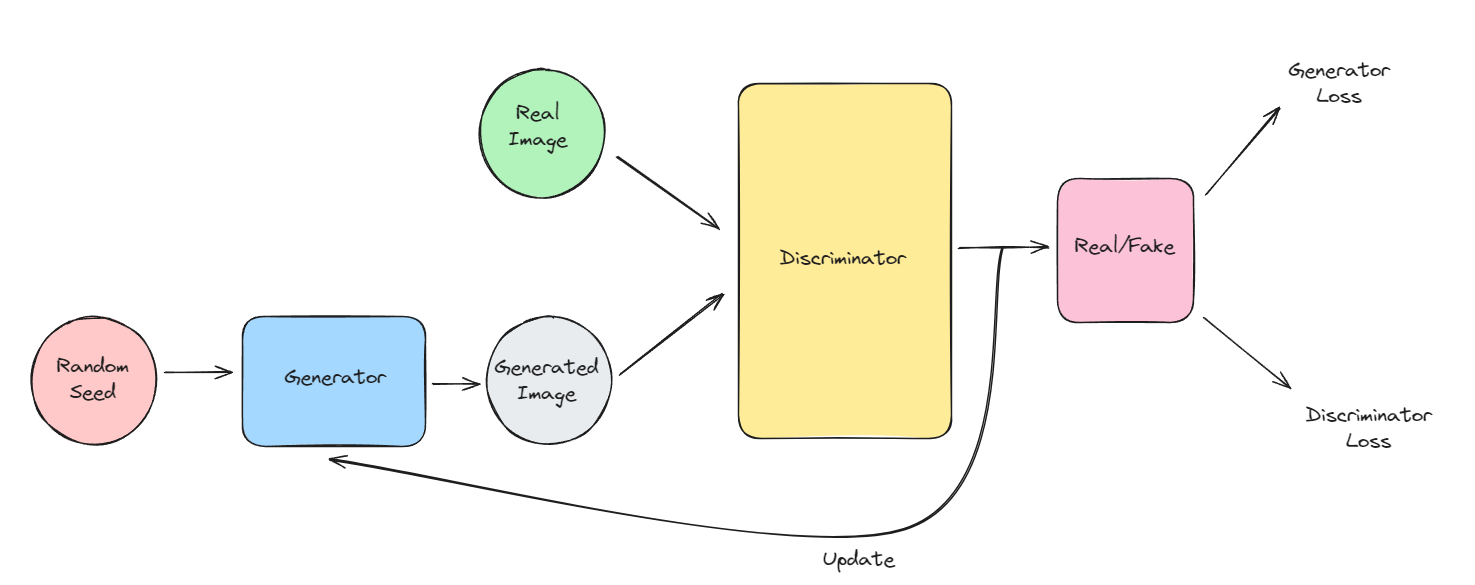
\includegraphics[width=1\textwidth]{images/gan_architecture.png}
    \caption{GAN mimarisi.}
    \label{fig:enter-label}
\end{figure}

\newpage

\subsection{Deep Convolutional GAN (DCGAN)}
2015 yılında Radford ve diğerleri tarafından yayınlanmıştır. GAN'dan farkı FC (tam bağlantılı) katmanlar yerine CNN kullanır. DCGAN, özellikle resimlerin üretilmesi üzerine odaklanmış olduğu için CNN mimarisini kullanır. CNN'ler genelde görüntüde korelasyon ararlar bu da DCGAN'ın resim ve videolar için daha uygun olduğu anlamına gelir. Kayıp fonksiyonu olarak "Binary Cross-entropy" kullanır.

\newpage

\subsection{Wasserstein GAN (WGAN)}
2017 yılında Arjovsky ve diğerleri tarafından tanıtılmıştır. Eğitimin kararlılığını artırmak için Wasserstein Distance (Wasserstein Mesafesi) kullanır. Bu daha kararlı ve düzgün bir gradyan akışı sağlar.  Wasserstein mesafesi, iki dağılım arasındaki en küçük taşıma maliyetini ölçer. Bu, bir dağılımı diğerine dönüştürmek için gereken minimum ortalama maliyeti ifade eder. Taşıma maliyeti, her bir parçacığın bir noktadan diğerine taşınması için gereken ortalama maliyettir. Wasserstein mesafesi, üretilen görüntülerin gerçek veri dağılımına ne kadar yakın olduğunu ölçer. Mode Collapse (mod çakışması) ve vanishing gradients (kaybolan gradyanlar) problemini çözmüştür. Mod çakışması, generator modelin çıktısının gerçek veri dağılımının yalnızca belirli bir alt kümesini yansıtmasıdır. Generator ağın her yinelemesinde discriminator ağın belirli bir alt kümeye aşırı uyum sağlaması sonucu oluşur. Kaybolan gradyanlarda ise Discriminator ağ, generator modelin ürettiği örnekleri kolayca ayırt edebilirse, generator model daha güvenli örnekler üretmeyi tercih edebilir. Bu da çeşitlilik eksikliğine neden olur.

\newpage

\subsubsection{Lipschitz Constraint}
WGAN formülasyonunda, modelin üretimindeki kararlılığın artırılması için discriminator ağın Lipschitz sürekli olduğunu garanti eden bir kısıtlama getirilmiştir. Lipschitz sürekliliği bir fonksiyonunun davranışının istikrarlı ve tahmin edilebilir olmasını sağlar. Bir fonksiyon, Lipschitz sürekliliğini sağlıyorsa, bu fonksiyonun davranışı belirli bir ölçüde "düzenli" olarak kabul edilir. Ancak, WGAN'da bu kısıtlamanın uygulaması zor olabilir. Hiperparametre "C" doğru ayarlanmadığında model düşük kaliteli görüntüler üretebilir.

\newpage

\subsection{Wasserstein GAN with Gradient Penalty (WGAN-GP)}
Gulrajani ve arkadaşları tarafından tanıtılmıştır. Eğitim sırasında Lipschitz kısıtlamasını elde etmek için Gradient Penalty (Gradyan Cezası) yöntemini kullanmasıdır. Gradient Penalty, discriminator ağı eğitiminde Lipschitz sürekliliğini zorlamak için ek bir terim olarak kullanılır. Gradient Penalty, discriminator ağın gradientlerinin normunu cezalandırarak çalışır. Bu, discriminator ağın gradyanlarının belirli bir sınıra yakın olmasını ve böylece Lipschitz sürekliliğini sağlamasını sağlar.

\newpage

\subsection{Conditional GAN (cGAN)}
Generator modelin belirli bir koşula göre (bir sınıf etiketi) öğrenilmesini sağlar. cGAN'da discriminator ağ, gerçek ve üretilen görüntü arasındaki farkı belirlerken bir koşul vektörünü ele alır ve bu vektörü göz önünde bulundurarak sınıflandırma yapar. Normal bir GAN modelinde gizli vektör eşlemesinin görüntünün gerçek özellikleriyle nasıl ilişkili olduğunu bilmiyoruz, bu nedenle bir "kara kutu" gibidir. Belirli sonuçlar elde etmek için bu özellikleri manipüle edemeyiz. Görüntü rastgele bir gürültüden oluşur. cGAN bu sorunu giderir.

\newpage

\subsection{Pix-to-Pix}
cGAN'ın bir türevidir. Bir görüntüden diğerine çeviri yapmak için kullanılır. Bir giriş görüntüsü alır ve bu giriş görüntüsünü belirli bir çıktı formatına çevirir. 

\newpage

\subsection{Cycle-Consistent GAN (CycleGAN)}
Bi görüntüden diğerine çeviri yapmak için kullanılır. Pix-to-pix gibi doğrudan eşleştirilmiş eğitim verilerine ihtiyaç duymaz. Bunun yerine "unsupervised learning (denetimsiz öğrenme)" prensibini kullanır. Cycle Consistency Loss, dönüşüm yapılırken orijinal görüntünün yeniden oluşturulmasını zorunlu kılar. Yani bir görüntü bir dönüşüme uğradıktan sonra tekrar orijinal hale geldiğinde, başlangıç ve sonuç arasında bir tutarlılık sağlar. Pix-to-pix'e kıyasla daha maliyetli ve zaman alıcı bir eğitim sunar. Renk ve doku değişikliklerini içeren çeviri görevlerinde yöntem genellikle başarılıdır. Örneğin at-zebra, elma-portakal dönüşümü.

\newpage

\subsection{Super Resolution GAN (SRGAN)}
2017 yılında Ledig ve diğerleri tarafından yayınlanmıştır. Düşük çözünürlüklü (Low-Resolution - LR) giriş görüntülerini yüksek çözünürlüklü (High-Resolution - HR) görüntülere dönüştürmeyi amaçlar. Generator, düşük çözünürlüklü giriş görüntüsünü alır ve bunu yüksek çözünürlüklü bir çıktıya dönüştürmeye çalışır. Sub-pixel convolution kullanır. Sub-pixel convolution, giriş görüntüsünü daha yüksek boyuta genişletmek yerine, gizli katmanlarda işlenirken yüksek boyutlu bir tensör oluşturur. Daha sonra bu tensör, bir kanal grubunu, pikselleri birleştirerek daha büyük bir tensör oluşturmak için yeniden boyutlandırır.

\newpage

\subsection{Enhanched Super Resolution GAN (ESRGAN)}
2018 yılında X. Wang ve diğerleri tarafından tanıtılmıştır. SRGAN'ın geliştirilmiş bir versiyonudur. ESRGAN'da, perceptual loss, content loss gibi özel kayıp fonksiyonları kullanılabilir. Bu kayıp fonksiyonları, üretilen görüntülerin daha fazla detay ve daha gerçekçi olmasını sağlamak için kullanılır. ESRGAN, transfer learning kullanarak önceden eğitilmiş bir VGG19 modelinin özelliklerini kullanabilir. Bu, generator ağın daha iyi sonuçlar elde etmek için daha fazla bilgiye erişmesini sağlar.

\newpage

\subsection{Progressive Growing of GAN (ProGAN)}
2017 yılında NVIDIA tarafından tanıtılmıştır. GAN'ların eğitimini aşamalı olarak gerçekleştiren ve daha yüksek çözünürlüklü görüntülerin üretimesini sağlayan bir modeldir. Düşük çözünürlüklü görüntülerden başlayarak yavaş yavaş daha yüksek çözünürlüklü görüntülere geçiş yapar. İlk olarak, generator ağ düşük çözünürlüklü görüntüleri üretmek için eğitilir. Her aşamada, generator ve discriminator ağ daha fazla katman ekler. Transfer learning yöntemlerini kullanarak önceki aşamalarda öğrenilen bilgileri daha sonraki aşamalara aktarır.

\newpage

\subsection{StyleGAN}
2018 yılında NVIDIA tarafından tanıtılmıştır. Yüksek kaliteli ve yüksek çözünürlüklü insan yüzü ve diğer görsel içeriklerin üretilmesi için kullanılır.

\newpage

\subsection{Vector Quantized GAN (VQGAN)}
Görsel verilerin temsillerini kodlamak ve yeniden oluşturmak için kullanılır. Giriş olarak verilen görsel veri üzerinde CNN kullanarak özellik çıkarımı yapılır. Elde edilen özellikler vektör kuantizasyonundan geçilir. Vektör kuantizasyonu, özellik vektörünü sabit bir sayıda semantik olarak anlamlı kümelerden birine atar. Bu, özellik vektörünün boyutunu azaltır ve daha basit bir temsil elde edilmesini sağlar. Kuantize edilmiş vektör, bir kodlayıcı kullanılarak daha düşük boyutlu bir vektöre kodlanır. Bu, görüntünün daha düşük boyutlu bir temsilini oluşturur. Kodlanmış vektör, bir dekoder kullanılarak yeniden oluşturulur. Bu, orijinal görüntünün yeniden oluşturulmasını sağlar. 

\newpage

\subsection{GauGAN}
NVIDIA tarafından geliştirilmiştir. Görüntülerin segmentasyonunu ve sentezini geliştirmek için kullanılır. Temel fikri, basit bir çizimle başlayarak karmaşık ve gerçekçi görüntüler oluşturmaktır. Kullanıcı, bir çizim arayüzü üzerinden basit bir çizim oluşturur. Çizim, farklı renklerle ve şekillerle temsil edilen nesneleri içerir. GauGAN, kullanıcının çizimini alır ve farklı nesneleri otomatik olarak tanımlar ve segmente eder. Bu, çizimin her bölgesinin hangi nesneye ait olduğunu belirlemek için bir segmentasyon aşamasını içerir. GauGAN, her bir nesne için bir özellik haritası oluşturur. Bu özellik haritaları, her bir nesnenin geometrik şeklini, renklerini ve diğer özelliklerini temsil eder. Her bir özellik haritası, o nesnenin piksel düzeyinde ayrıntılı bir temsilini içerir. GauGAN, özellik haritalarını birleştirir ve gerçekçi bir görüntü oluşturur.

\newpage

\subsection{Generative Face Completion (GFP-GAN)}
Yüz görüntülerinin tamamlanması ve restore edilmesi için kullanılır. Yarı eksik veya bozulmuş bir yüz görüntüsünü alır. Eksik yüz görüntüsünü bir latent uzayda kodlamak için bir kodlayıcı kullanır. Bu, eksik görüntünün temsilini elde etmek ve işlemek için bir vektör oluşturur. Kodlanmış eksik görüntü vektörü bir dekoder kullanarak tamamlanır. 

\newpage

\subsection{Auxiliary Classifier GAN (ACGAN)}
Standart GAN mimarisine ek olarak 1 adet sınıflandırıcı eklenmiştir. Bu sınıflandırıcı, üretilen verinin hangi sınıfa ait olduğunu tahmin etmeye çalışır. Böylece, üretilen verinin hem gerçekçi olması hem de belli bir sınıfa ait olması sağlanır.

\begin{itemize}
    \item \textbf{Adversarial Loss}: Üretilen örneğin gerçek mi sahte mi olduğunu ölçer.
    \item \textbf{Auxiliary Loss}: Üretilen örneğin hangi sınıfa ait olduğunu ölçer.
\end{itemize}

\newpage

\subsection{Boundary Equilibrium GAN (BEGAN)}

BEGAN, bir denge noktası (equilibrium point) ile generator ve discriminator arasındaki dengeyi kurar. Böylece, modelin overfitting ve mode collapse gibi sorunlarla karşılaşma olasılığı azalır. 

\subsubsection{Çalışma Adımları}

\begin{enumerate}
    \item Eğitime başlarken, denge parametresi küçük bir değere ayarlanır. 
    \item Ayırıcının yaptığı hata kullanılarak, denge parametresi güncellenir. Eğer ayırt edici çok fazla hata yapıyorsa, denge parametresi artıralarak üreticiye daha fazla özgürlük verir. Eğer ayırt edici çok az hata yapıyorsa, denge parametresi azaltılarak üretici daha kısıtlanır.
\end{enumerate}

\newpage

\subsection{Boundary-Seeking GAN (BSGAN)}

BSGAN'ın temel farkı, Discriminator'un kararlarının olasılık dağılımının sınırlarında toplanmasını sağlamasıdır. Bu, eğitim sırasında üretilen verinin kalitesini artırmakta ve daha stabil bir eğitim süreci sunmaktadır.

\subsubsection{Çalışma Adımları}

\begin{enumerate}
    \item Rastgele gürültüden görüntüler üretilir.
    \item Ayırıcı, üretilen örneklerin gerçek olup olmadığını belirlerken aynı zamanda bu örneklerin veri dağılımındaki konumunu da değerlendirir.
    \item Ayırıcı, üretilen örneklerin veri dağılımının sınırlarına daha yakın olduğunu tespit ederse, üretiyici bu yönde teşvik eder.
    \item Üretici ve ayırt edici arasındaki bu etkileşim, bir denge içinde sürdürülür.
\end{enumerate}

\newpage

\subsection{Cluster GAN (Clustering-aware GAN)}

Kümeleme ve jeneratif modellemeyi birleştirir. Cluster GAN, hem gerçek verilerin dağılımını öğrenmek hem de veriyi kümelere ayırmak amacıyla tasarlanmıştır. Gerçek verilerin altında yatan gizli yapıları öğrenirken, üretilen veriyi bu yapılara göre kategorize ederek yüksek kalitede örnekler oluşturmayı hedefler. İçerisinde Generator ve Discriminator'a ek olarka bir adet Encoder bulunur. Bu encoder, gerçek veriyi gizli uzaya kodlayarak, bu verilerin nasıl dağıldığını öğrenir.

\subsubsection{Çalışma Adımları}

\begin{enumerate}
    \item Rastgele gürültüden görüntüler üretilir.
    \item Kümeleme modülü, üretilen örnekleri belirli sayıda kümeye ayırır.
    \item Kümeleme sonuçları, hem üreticiye hem de ayırt ediciye geri beslenir. Üretici, örneklerini daha iyi tanımlanmış kümelere üretmeye çalışırken, ayırt edici de bu kümeleri ayırt etmeye çalışır.
\end{enumerate}

\newpage

\subsection{Context-Conditional GAN (CCGAN)}

Modelin veri üretim sürecinde belirli bir bağlamı (context) dikkate almasını sağlar. Bu model, belirli bir koşula göre veri üretebilir. Bağlam, modelin veri üretiminde dikkat etmesi gereken koşullu bilgiyi sağlar. Bu, metin, sınıf etiketi, görüntü özelliği gibi herhangi bir bağlamsal bilgi olabilir. Üretici, girdiye yalnızca rastgele bir gürültü vektörü değil, aynı zamanda belirli bir bağlamda koşullu bilgi de alır. Üretici, bu bilgiyi dikkate alarak koşula uygun veri üretir. 

\newpage

\subsection{Context-Encoder GAN (CEGAN)}

Eksik veya kısmı verileri tamamlama (inpainting) problemlerinde kullanılan bir GAN çeşididir. Eksik bir girdiyi kullanarak bu eksikliği doldurmak ve orijinal tam veri ile uyumlu bir çıktı üretmek üzere tasarlanmıştır. Özellikle gürültü tamamlama, ses veya diğer veri türlerinin eksik kısımlarının yeniden oluşturulmasında etkilidir. Bağlamsal bilgiyi dikkate alarak eksik veriyi tahmin etmeye çalışır.

\newpage

\subsection{Coupled GAN (CoGAN)}

İki farklı ama ilgili veri dağılımını öğrenmek ve bu iki dağılımı eşleştirmek amacıyla kullanılan bir GAN türüdür. CoGAN, iki farklı veri kümesinden benzer yapılsal özelliklere sahip veriler üretmek için tasarlanmıştır. Bu yöntem, iki GAN'ın ağırlık paylaşımı yoluyla birbirleriyle senkronize çalışmasıyla, çiftler halinde uyumlu veri üretimi sağlar. Bu GAN'lar birbirinden bağımsız çalışsa da, belirli katmanlar arasında ağırlık paylaşımı yaparak iki veri kümesi arasındaki ortak özellikleri öğrenirler. Bu mimaride, her iki GAN'ın Generator ve Discriminator'ları bulunur, ancak belirli katmanlar ortak kullanılır. 

\newpage

\subsection{Disco GAN}

İki farklı veri kümesi arasındaki ilişkili fakat farklı özellikleri öğrenmeye ve dönüştürmeye odaklanan bir GAN türüdür. İki farklı alan arasında birbiriyle uyumlu veriler üreterek, iki veri kümesi arasında çift yönlü dönüştürme yapmayı hedefler. Örneğin, bir alandaki veriyi diğer alana dönüştürme ve ardından bu dönüşümü tekrar orijinal alana geri döndürme işlemini gerçekleştirir. Disco GAN, çembersel bir kayıp fonksiyonu kullanır. Bu sayede, bir veri önce bir domaine dönüştürülüp sonra tekrar ilk domainine geri döndürüldüğünde, başlangıçtaki veriye mümkün olduğunca yakın bir sonuç elde edilmesi hedeflenir.

\newpage

\subsection{Deep Regret Analytic GAN (DRAGAN)}

Temel amacı, GAN'larda karşılaşılan eğitim dengesizliklerini ve başarısızlıkları engellemektedir. Bu dengesizlikler genellikle ayrıştırıcı ağın çok hızlı bir şekilde güçlenmesi ve üretici ağın iyi öğrenememesi durumlarında ortaya çıkar. DRAGAN, bu sorunu çözmek için ayrıştırıcıya, eğitim sırasında ek regülarizasyon teknikleri uygular.  Gradient Regularization (Gradient Penalty) sayesinde ayrıştırıcının eğitimi sırasında hatalı veya aşırı güçlü öğrenmesi engellenir. Böylece, ayrıştırıcı çok hızlı şekilde öğrenip üreticiyi başarısız kılacak kadar güçlü hale gelmez. 

\newpage

\subsection{DualGAN}

iki yönlü görntü dönüşümleri için kullanılır. Çift yönlü dönüşümler, bir görüntü alanından diğerine ve ardından tekrar geri dönüşümü mümkün kılmayı hedefler. Örneğin siyah-beyaz bir görüntüyü renklendirmek ve ardından bu renklendirilmiş görüntüyü tekrar siyah-beyaz hale getirmek gibi görevlerde kullanılır. Cycle Consistency Loss, iki veri alanı arasındaki dönüşümlerin mantıklı olmasını sağlar. Dönüştürülmüş veri, tekrar orijinal veri alanına geri çevrilir. Örneğin $X \rightarrow Y \rightarrow X$ dönüşümü, başlangıçtaki X görüntüsüne mümkün olduğunca yakın olmalıdır. Bu, "cycle consistency loss" ile ölçülür.

\newpage

\subsection{Energy-based GAN (EBGAN)}

EBGAN, klasik GAN yapısını enerji temelli bir yaklaşımla yeniden formüle eden bir modeldir. Ayrıştırıcıyı bir enerji fonksiyonu olarak ele alır ve bu fonksiyonun çıktısının, bir veri örneğinin gerçek veya sahte olupğ olmadığını belirlediği bir enerji temelli model ortaya koyar. Ayrıştırıcı, bu enerji seviyesini minimize etmeye odaklanır. Gerçek veriler için enerji seviyesini düşürmeye çalışırken, sahte veriler için bu seviyeyi artırır. Ayrıştırıcının çıktısı, bir veri örneğinin "enerjisini" temsil eder. Bu enerji bir reconstruction loss (yeniden yapılandırma hatası) olarak yorumlanır. Gerçek verilerde bu hata daha düşük, sahte verilerde ise daha yüksek olacak şekilde optimize edilir.

\newpage

\subsection{Information Maximizing GAN (InfoGAN)}

Denetimsiz öğrenme ile anlamlı ve yorumlanabilir veri temsilleri elde etmeye odaklanır. InfoGAN, üretilen veriler üzerinde kontrol sahibi olmayı sağlar ve gizli değişkenlerin bazılarını anlamlı hale getirir. Bu, üretilen örneklerdeki belirli faktörlerin manipüle edilmesini mümkün kılar. Ayrıştırıcı, sahte veya gerçek verileri ayırt ederken aynı zamanda üreticinin ürettiği bilgiyi yeniden yapılandırmaya çalışır. Bu yeniden yapılandırma işlemi ile bilgi kaybı (mutual information) minimize edilir. Q ağı, ayrıştırıcı ile birlikte çalışarak bilgi vektörünün geri kazanılmasını sağlar. Verilen sahte örneklere göre bilgi vektörünü tahmin eder. 

\newpage

\subsection{Least Squares GAN (LSGAN)}

LSGAN'da ayrıştırıcıda kullanılan kayıp fonksiyonu binary cross entropy yerine ortalama kare hata (mean squared error) olarak değiştirilmiştir. Gerçek veriler için yüksek değerler, sahte veriler için düşük değerler üretir. LSGAN'da Discriminator'un çıktısı gerçeklik ve sahtelik arasındaki farkı ifade eder ve bu fark ortalama kare ile hesaplanır. Gerçek veriler için hedef değer 1, sahte veriler için hedef değer 0'dır. Ayrıştırıcının kaybı, gerçek ve sahte verilerin tahmin edilen değerleri ile bu hedef değerler arasındaki ortalama kare hatadır. Üreticinin amacı sahte veriler için tahmin ettiği değerlerin 1'e ne kadar yakın olduğunu sağlamak için kaybını minimize eder. Bu, üreticinin ayrıştırıcıyı daha iyi yanıltmasını sağlar.

\newpage

\subsection{Unified GAN for Image-to-Image Translation (UNIT)}

Birden fazla görüntü dönüşüm görevini tek bir modelle gerçekleştirebilen bir modeldir. Encoder, giriş görüntüsünü özellik haritalarına dönüştüren bir ağdır. Decoder, özellik haritalarını hedef alanda uygun bir görüntüye dönüştürür. Domain-Agnostic Encoder, hem kaynak hem de hedef alanlar için ortak bir encoder kullanılır. Bu, modelin genel özellikleri öğrenmesini sağlar. Domain-Specific Encoder, her bir alan için özel decoder kullanılır. Bu, her alanın özgüllüklerini yakalamak için gereklidir. Domain Classifier, üretilen görüntülerin hangi alana ait olduğunu tahmin eden bir bileşendir. Bu, alanlar arasındaki farklılıkları öğrenmeye yardımcı olur. 

\newpage

\subsection{Multimodal Unsupervised Image-to-Image Translation (MUNIT)}

Çok modlu ve denetimsiz görüntü şekil çevirisi için geliştirilmiş bir generatif modeldir. MUNIT, bir görüntünün stilini ve içeriğini ayırarak, çeşitli stiller arasında dönüşüm yapabilen ve çeşitli içeriklerle uyumlu olan bir model sunar. İçerik kodlayıcı (content encoder), girdi görüntüsünün içeriğini çıkarır ve içerik özelliklerini temsil eden bir vektör üretir. Stil kodlayıcı (style encoder), girdi görüntüsünün stil özelliklerini çıkarır ve stil özelliklerini temsil eden bir vektör üretir.

\subsubsection{Çalışma Adımları}

\begin{enumerate}
    \item Girdi görüntüsü, içerik ve stil kodlayıcıları tarafından işlenir. İçerik kodlayıcı görüntünün içeriğini temsil eden bir vektör oluştururken, stil kodlayıcı, stil özelliklerini temsil eden bir vektör oluşturur.
    \item İçerik vektörü ve stil vektörü, dönüşüm ağına (generator) beslenir. Dönüşüm ağı, bu bilgileri birleştirerek hedef stilde dönüştürülmüş bir görüntü üretir.
    \item Üretilen görüntüler, ayrıştırıcı tarafından değerlendirilir. Ayrıştırıcı, görüntülerin gerçekliği ve içerik-stil uyumu hakkında geri bildirim sağlar.
    \item İçerik kaybı, üretilen görüntünün içerik vektörünü kaynak içerik vektörü ile karşılaştırarak hesaplanır. Stil kaybı, üretilen görüntünün stil vektörünü hedef stil vektörü ile karşılaştırarak hesaplanır. Adversarial (gerçek-sahte) kayıp, ayrıştırıcı tarafından hesaplanan görüntülerin gerçekliğini değerlendirir.
    \item Hesaplanan hatalar kullanılarak üretici ve ayrıştırıcı ağları güncellenir.
\end{enumerate}

\newpage

\subsection{Pixel-wise Domain Adaption (PixelDA)}

Bir görüntü setinin başka bir kaynaktan başka bir kaynağa dönüştürülmesi gereken durumlarda kullanılır. Özellik çıkarıcı (feature extractor) ve uyum ağı (adaptation) networkten oluşur. Özellik çıkarıcı (feature extractor), görüntüleri işleyerek anlamlı özellikler çıkarır. Her iki alanda da (kaynak ve hedef) ortak bir temsil öğrenir. Uyum ağı (adaptation network), özellikleri her iki alan arasında uyumlu hale getirmek için çalışır. Bu ağ, kaynak ve hedef alanlardaki özelliklerin uyumlu olmasını sağlar. Bu iki alan arasındaki farklılıkları minimize etmeye çalışır.  Reconstruction Loss (Geri Dönüşüm Kaybı), özelliklerin doğru bir şekilde uyum sağladığını kontrol etmek için kullanılır. Bu kayıp, dönüştürülmüş görüntülerin kaynaktan hedef alana doğru bir şekilde haritalanıp haritalanmadığını kontrol eder. 

\subsubsection{Çalışma Adımları}

\begin{enumerate}
    \item Kaynak ve hedef görüntüler, özellik çıkarıcı tarafından işlenir. Bu, her iki alanda da ortak bir özellik temsilinin elde edilmesini sağlar.
    \item Özellikler, uyum ağı tarafından dönüştürülür. Bu, kaynak ve hedef alanlar arasındaki farklılıkları azaltmak için yapılır. Özelliklerin uyumlu hale gelmesi sağlanır.
    \item Dönüştürülmüş özellikler, kaynak görüntülerin hedef görüntülere dönüşümünü sağlar. Geri dönüşüm kaybı hesaplanır ve uyum ağı bu kaybı minimize etmek için eğitilir.
    \item Özelliklerin doğru şekilde çıkarıldığını ve sınıflandırıldığını kontrol eden bir sınıflandırma ağı kullanılır. Bu, modelin hedef alan üzerinde doğru sınıflandırmalar yapabilmesini sağlar.
    \item Özellik çıkarıcı, uyum ağı ve sınıflandırma ağı, geri dönüşüm ve sınıflandırma kayıplarına göre güncellenir.
\end{enumerate}

\newpage

\subsection{Relativistic GAN}

Relativistic GAN, gerçek ve sahte görüntüleri tek tek değerlendirmek yerine, bunları birbiriyle karşılaştırır. Bu yaklaşım, ayrıştırıcının daha iyi bir göreceli değerlendirme yapmasını sağlar. Relativistic Loss, ayrıştırıcının gerçek ve sahte görüntüler arasındaki göreceli farklı öğrenmesini sağlar.

\newpage

\subsection{Semi-Supervised GAN}

GAN içinde yarı denetimli öğrenmeyi kullanan bir modeldir. Bu model, etiketlenmiş ve etiketlenmemiş verilerle öğrenme sürecini destekler. SSGAN'de Discriminator ağı ayrıca sınıflandırma görevini de yerine getirir. Bu, Discriminator'un her görüntüyü hem gerçek/sahte hem de sınıf bilgisi açısından değerlendirmesini sağlar.

\newpage

\subsection{Softmax GAN}

GAN içinde Softmax fonksiyonunu kullanarak, özellikle sınıflandırma problemlerini çözme ve yüksek kaliteli veri üretme konusunda geliştirilmiş bir modeldir. Softmax GAN, klasik GAN mimarisine ek olarak Softmax fonksiyonunu kullanarak sınıflandırma işlevselliği ekler. Softmax Katmanı, Discriminator ağına entegre edilir ve verilerin farklı sınıflara ait olma olasılıklarını hesaplar. Softmax fonksiyonu, bir dizi olasılığı normalize ederek, her bir sınıf için olasılıkları toplar ve bu olasılıkların toplamı 1 olur. Discriminator ağı, gerçek ve sahte verilerden özellikler çıkarır. Bu özellikler, Softmax katmanı tarafından sınıflandırma yapılacak şekilde işlenir. Generator ve Discriminator ağları, Softmax fonksiyonunun hesapladığı sınıf kaybı ve gerçek/sahte kayıplarına göre güncellenir.

\newpage

\subsection{Star GAN}

Çeşitli veri kümeleri üzerinde çoklu alanlarda (domain) verileri dönüştürmek için kullanılan bir modelidir. StarGAN, tek bir model kullanarak farklı alanlarda veri dönüştürme işlemlerini gerçekleştirebilir. Domain Classifier (Alan Sınıflayıcı), üretici ve Discriminator'den bağımsız olarak çalışır ve verilerin hangi alana ait olduğunu tahmin eder. 

\newpage

\subsection{Adaptive Boosting GAN (AdaGAN)}

Boosting yöntemini kullanan bir GAN türüdür. Temel olarak zayıf generatorlerin ardışık olarak eğitildiği ve bu generatorlerin oluşturduğu zayıf modellerin sonunda güçlü bir model oluşturmak için birleştirildiği bir yapıyı benimser. Ardışık olarak eğitilen birden fazla generator modeli vardır. Her generator, veri kümesinin bir kısmını daha iyi modellemeye odaklanır. Her generatorün oluşturduğu örnekleri değerlendiren ve bu değerlendirmelere göre generatorlerin ağırlıklarını güncelleyen bir ayrıştırıcı ağ bulunur. Generatorler arasındaki adaptif ağırlıklandırma (adaptive weighting) sistemi, her generatorun başarı oranına göre güncellenir. Bu sayede daha kötü performans gösteren generatorler, diğer generatorler tarafından telafi edilir. 

\subsubsection{Çalışma Adımları}

\begin{enumerate}
    \item İlk generator, gerçek veri ve rastgele gürültüden türetilen sahte veri arasında ayrım yapmaya çalışan bir discriminator yardımıyla eğitilir.
    \item İlk generator eğitildikten sonra, generatorün başarısız olduğu örnekler tespit edilir ve bu örneklere daha yüksek ağırlıklar verilir. Bu süreç, boosting'in ana fikri olan hatalı örneklerin ağırlıklarının artırılmasına dayanır.
    \item Yüksek ağırlıklandırılmış örnekler üzerinde daha iyi performans gösterecek şekilde sonraki generatorler eğitilir. Her generator, bir önceki generatorün başarısız olduğu bölgeleri hedef alır.
    \item Eğitilen tüm generatörler, ağırlıklarına göre birleştirilir ve güçlü generator model oluşturulur.
\end{enumerate}

\newpage

\subsection{Balanced Consistency Regularization (bCR)}

GAN için geliştirilmiş bir tutarlılık düzenleme (consistency regularization) tekniğidir. Discriminator'un daha dengeli ve tutarlı geri bildirimler sağlamasını hedefler, böylece Generator'un daha doğru ve gerçekçi örnekler üretmesini teşvik eder. Consistency Regularization Term, Discriminator'un benzer girişler için tutarlı çıktılar üretmesini sağlamak amacıyla kayıp fonksiyonuna eklenir. Bu sayede, Discriminator, aynı veya benzer görüntüler için tutarlı kararlar verir.  

\[ \text{BCR} = \lambda \cdot \mathbb{E}\left[\|f(x) - f(\hat{x})\|_2^2\right] \]

\begin{itemize}
    \item $f(x)$: Modelin x girdi vektörüne verdiği çıkış vektörü.
    \item $f(\hat{x})$: Modelin değiştirilmiş x girdi vektörüne verdiği çıkış vektörü.
    \item $\mathbb{E}\left[\|f(x) - f(\hat{x})\|_2^2\right]$: İki vektör arasındaki L2 normunun, yani Euclidean mesafesinin, karesi.
\end{itemize}

\newpage

\subsection{BigGAN}

Yüksek kaliteli doğal görüntülerin üretilmesi için geliştirilmiş bir modeldir. Sınıf koşullu generator kullanır. Yani, üretilen görüntüler belirli bir sınıfa ait olacak şekilde kontrol edilebilir. Spectral Normalization tekniğini kullanarak ağırlıkları kontrol eder. Spectral Normalizatoin, Discriminator'un spektral normlarını sınırlayarak, ağın kararlılığını sağlar. Böylece overfitting'in görülmesini azaltmaya çalışır.

\newpage

\subsection{ConSinGAN}

Tek bir görüntüden çeşitli ve yüksek çözünürlükte görüntüler üreten bir modeldir. ConSinGAN, yalnızca tek bir örnek görüntüden öğrenme kapasitesine sahiptir. ConSinGAN’in mimarisi, ölçekler arasında ilerleyerek görüntü üretimini sağlayan çok katmanlı bir yapıyı içerir. Bu mimaride, Generator ve Discriminator ağları, farklı çözünürlüklerde görüntüler üretmek ve değerlendirmek için kademeli olarak eğitilir. Bu süreç, çeşitli çözünürlüklerde daha küçük ölçeklerde başlayan ve en sonunda tam çözünürlüklü görüntüler üreten bir yapı ile gerçekleştirilir. Koşullu Yürütme (Conditional Execution) ile Generator, önceki çözünürlükte üretilen görüntüyü giriş olarak alır ve bunu bir sonraki çözünürlüğe genişletir. Bu, Generator'un her aşamada daha karmaşık ve yüksek çözünürlüklü görüntüler üretebilmesini sağlar. Her çözünürlük katmanında eklenen rastgele gürültü, çeşitliliğin artırılmasını ve Generator'un farklı çıktılar üretebilmesini sağlar.

\begin{itemize}
    \item \textbf{Multi-Scale Generator (Çok Ölçekli Generator)}: ConSinGAN, görüntüleri farklı çözünürlüklerde oluşturmak için çok ölçekli bir Generator ağına sahiptir. Her bir ölçek, önceki ölçekten elde edilen çıktıyı kullanarak bir sonraki ölçekli görüntüyü üretir.
    \item \textbf{Multi-Scale Discriminator (Çok Ölçekli Discriminator)}: Discriminator ağı da benzer şekilde çok ölçekli çalışır. Her bir ölçek, o çözünürlükte üretilen görüntüyü gerçek veya sahte olarak değerlendirir.
\end{itemize}

\subsubsection{Çalışma Adımları}

\begin{enumerate}
    \item Tek bir giriş görüntüsü, en küçük çözünürlükten en büyük çözünürlüğe kadar olan bir dizi ölçeğe bölünür. Bir görüntü önce çok küçük bir çözünürlükte işlenir, ardından daha yüksek çözünürlüklere doğru kademeli olarak genişletilir
    \item Eğitim süreci, en küçük çözünürlükteki Generator ve Discriminator çiftini eğitmekle başlar. Bu çift, görüntünün düşük çözünürlüklü bir versiyonunu üretir ve discriminator bu görüntüyü gerçek veya sahte olarak değerlendirir. Bu süreç, her bir ölçek için tekrarlanır ve her adımda Generator bir önceki çözünürlükte üretilen görüntüyü genişleterek daha büyük bir görüntü üretir.
    \item Her bir ölçek için Generator, ek rastgele gürültü alır. Bu gürültü, Generator'un daha çeşitli ve benzersiz görüntüler üretmesini sağlar.
    \item Generator her bir çözünürlükte önceki çözünürlükte üretilen görüntüyü giriş olarak alır. Bu nihai yüksek çözünürlüklü görüntünün oluşturulmasını sağlar.
\end{enumerate}

\newpage

\subsection{EqGAN-SA}

Mekansal farkındalık (spatial awareness) kullanarak GAN'lardaki dengesizlik sorunlarını gidermeyi amaçlamaktadır. Generator, mekansal bilgiyi de dikkata alarak görüntü üretir. Discriminator ise mekansal farkındalığa sahiptir ve bu sayede sadece genel farkları değil, aynı zamanda mekansal özellikleri de değerlendirebilir. Generator ve Discriminator mekansal farkındalık kaybı (spatial awareness loss) kayıp fonksiyonunu optimize ederken mekansal bilgiyi dikkate alır.

\subsubsection{Çalışma Adımları}

\begin{enumerate}
    \item Generator, rastgele gürültüden başlar ve mekansal farkındalık katmanı kullanarak görüntüleri üretir. Aynı zamanda, bu katman, mekansal özellikleri daha iyi yakalayabilmek için Generator'un çıktısını detaylandırır.
    \item Discriminator, mekansal farkındalık katmanından gelen veriyi kullanarak, Generator tarafından üretilen görüntüleri analiz eder.
    \item Dengeleme mekanizması, Generator ve Discriminator arasındaki dengeyi sağlamak için devreye girer. Bu mekanizma, iki ağı da eşit seviyede eğiterek birinin diğerinden çok daha hızlı veya yavaş öğrenmesini engeller.
    \item Generator ve Discriminator, mekansal farkındalık kaybını minimize etmeye çalışır.
    \item Generator, Discriminator'den gelen bilgiyi alır ve bu bilgilere dayanarak görüntüleri iyileştirir. Bu süreç, dengeyi koruyarak tekrarlanır.
\end{enumerate}

\newpage

\subsection{f-GAN}

GAN'ın temel problemlerinden olan divergence ölçümünü ele alır ve bu ölçümü minimize ederek Generator'un daha gerçekçi veriler üretmesini sağlar. f-GAN'da, Discriminator'un amacı yalnızca gerçek veya sahteyi ayırt etmek değildir; aynı zamanda belirli bir divergence minimize edecek şekilde optimize edilir. f-Divergence, iki olasılık dağılımı arasındaki farklılığı ölçen bir fonksiyondur. f-GAN, bu fonksiyonları kullanarak Genreator ve gerçek veri dağılımı arasındaki farklılığı minimize eder. 

\newpage

\subsection{Generative Adversarial Paralellization (GAP)}

GAN'ların eğitim sürecini daha hızlı ve verimli hale getirmek amacıyla paralelleştirme tekniklerini kullanır. GAP, birden fazla paralel Generator'un aynı anda eğitilmesine izin verir. Bu Generator'ler, veri setinin farklı bölümlerinde çalışır ve aynı zamanda farklı türde veriler üretebilirler. GAP, birden fazla paralel Discriminator'ler kullanarak Generator'lerin ürettiği verilerin doğruluğunu test eder. Generator'lerin ürettiği veriler üzerinde farklı kriterler değerlendirme yapabilirler. Paralel Generator'ler ve Discriminator'ler arasındaki koordinasyonu sağlamak için bir kontrol mekanizması kullanılır. Bu mekanizma, Generator'lerin ve Discriminator'lerin senkronize çalışmasını ve verimli bilgi paylaşımını sağlar.

\begin{itemize}
    \item \textbf{Master Generator}: Generator'lerin genel yönünü ve stratejisini belirler. Ana Generator, paralel Generator'lerden gelen geri bildirime göre kendini optimize eder.
    \item \textbf{Sub-Generators}: Veri setinin belirli bölümlerini işlerler. Alt Generator'ler, veri setini farklı perspektiflerden ele alarak daha geniş bir veri çeşitliliği sağlar.
    \item \textbf{Master Discriminator}: Paralel Discriminator'lerden gelen bilgileri bir araya getirir ve Generator'lerin genel performansını değerlendirir.
    \item \textbf{Sub-Discriminator}: Üretilen verileri farklı kriterler üzerinden değerlendirir. Bu Discriminator'ler, Generator'lerin sahte ve gerçek verileri ayırt etmesine yardımcı olur.
    \item \textbf{Coordination Mechanism}: Paralel Generator'ler ve Discriminator'ler arasında veri alışverişini ve senkronizasyonu sağlar.
\end{itemize}

\newpage

\subsection{Geometric GAN (GGAN)}

GAN modellerinin eğitimini geometrik özelliklere dayalı olarak optimize etmeye çalışan bir GAN türüdür. Discriminator'un karar sınırlarını optimize eden geometrik bir düzenleme (geometric measure) kullanır. 

\newpage

\subsection{Laplacian Pyramid GAN (LAPGAN)}

LAPGAN, düşük çözünürlüklü bir görüntüyü kademeli olarak yüksek çözünürlüklü hale getirir. Bu süreç, Laplace piramidi olarak bilinen çok seviyeli bir görüntü temsil yöntemine dayalıdır. Bir görüntü, Laplace piramidi yöntemiyle farklı çözünürlük seviyelerine ayrılır. Her seviye, bir önceki seviyedeki düşük çözünürlüklü görüntüden türetilir ve bu seviyeye ait detayları içerir. LAPGAN, her çözünürlük seviyesinde bir Generator kullanır. Bu Generator'ler, bir önceki seviyede üretilen görüntüyü alır ve bu görüntüyü daha yüksek bir çözünürlükte yeniden üretir. Her Generator, bir önceki çözünürlük seviyesinin detaylarını ekler. Her çözünürlük seviyesi için ayrı bir Discriminator modeli bulunur. Bu Discriminator'ler, Generator'lerin ürettiği görüntülerin gerçek mi yoksa sahte mi olduğunu ayırt etmek için kullanılır. Discriminator'ler, her çözünürlük seviyesinde Generator'leri zorlayarak daha gerçekçi görüntüler üretilmesine yardımcı olur. 

\newpage

\subsection{Margin Adaptation for GAN (MAGAN)}

Generator ve Discriminator arasındaki yarışmayı daha stabil hale getirmek için "marjin adaptasyonu (margin adaptation)" yöntemini kullanır. Marjin adaptasyonu, Discriminator'un karar sınırını (yani marjini), dinamik olarak ayarlayarak Generator'un daha iyi öğrenmesini sağlar. Discriminator, sahte veriler üzerinde eğitildikçe, belirli bir marjin (sınır) içinde bu verileri sınıflandırmaya çalışır. Eğer Generator'un ürettiği veriler Discriminator tarafından kolayca ayırt ediliyorsa, bu marjin daraltılır; eğer Discriminator zorlanıyorsa, marjin genişletilir.

\newpage

\subsection{Mode Regularized GAN (MRGAN)}

MRGAN (Mode Regularized Generative Adversarial Networks), GAN’ların (Generative Adversarial Networks) mod çöküşü (mode collapse) sorununu çözmek için tasarlanmış bir modeldir. Mod çöküşü, Generator'un sınırlı sayıda veri modunu (örneğin, görüntü varyasyonlarını) öğrenmesi ve bu nedenle sadece belirli türde veriler üretmesi durumudur. MRGAN, Generator'un daha geniş bir veri dağılımını öğrenmesini sağlamak amacıyla mod düzenlemesi (mode regularization) mekanizmasını kullanır. Mod Düzenleyici Terim (Mode Regularization Term), Generator'un veri modlarını daha geniş bir şekilde kapsamasını sağlamak amacıyla Generator'un kayıp fonksiyonuna eklenir. 

\newpage

\subsection{Multi-Scale Gradients for GAN (MSGGAN)}

Eğitim sırasında çok ölçekli gradyanlar kullanır. Çok ölçekli gradyanlar, Generator'un her çözünürlük seviyesinde nasıl performans gösterdiğini değerlendiren gradyanlar üretir.

\newpage

\subsection{Relativistic Average GAN (RaGAN)}

Relativistic Discriminator adı verilen bir mekanizmayı kullanır. Relativistic Discriminator, sahte verilerin ne kadar gerçek olduklarını değerlendirmek yerine, gerçek verilerin sahte verilere kıyasla ne kadar gerçek olduğunu değerlendirir.

\newpage

\subsection{Self-Attention GAN (SeAtGAN)}

Self-Attention mekanizmasını kullanarak Generator ve Discriminator'un daha uzun menzilli bağımlılıkları öğrenmesini sağlar. Self-Attention, modelin görüntüdeki uzak pikseller arasındaki ilişkiyi anlamasına ve bu sayede daha tutarlı ve kaliteli sahte veriler üretmesini sağlar. 

\newpage

\subsection{SphereGAN}

Mod çökmesi (mode collapse) gibi sorunları küresel (sphere) bir proje üzeirnde geometrik moment uyumlaması ile çözer. SphereGAN, veri dağılımlarını geometrik momentlerle tanımlayarak, Generator'un bu dağılımları daha doğru bir şekilde öğrenmesini ve modellemesini sağlar. Generator, verileri bir küresel yüzey üzerine projekte eder. Bu, veri dağılımlarının geometrik bir yapıya uygun hale gelmesini sağlar ve mod çökmesini engeller. Discriminator, verilerin geometrik momentlerini hesaplar ve bu momentleri kullanarak Generator'un ürettiği verileri değerlendirir.

\newpage

\subsection{Stacked GAN (SGAN)}

SGAN, birden fazla Generator ve Discriminator katmanını ardışık olarak bir araya getirerek, düşük çözünürlüklü bir görüntüden başlayarak adım adım daha yüksek çözünürlüklü ve detaylı bir görüntü oluşturmayı hedefler. Bu mimari, özellikle karmaşık ve yüksek çözünürlüklü görüntülerin üretimi için kullanışlıdır. İlk Generator (G1) düşük çözünürlüklü bir görüntü üretir. İlk Discriminator (D1) bu görüntüyü gerçek düşük çözünürlüklü görüntülerle karşılaştırır ve gerçek ya da sahte olduğunu belirler. Her ardışık Generator, önceki Generator'un ürettiği görüntüyü alır ve bunu daha yüksek çözünürlüklü bir görüntüye dönüştürmeye çalışır. Her Generator ve Discriminator çifti, bir önceki katmanın çıktısını alır ve üzerine daha fazla detay ekler. Son Generator, en yüksek çözünürlüklü görüntüyü üretir. Bu, başlangıçtaki düşük çözünürlüklü görüntünün aşamalı olarak iyileştirilmesiyle elde edilir. 

\newpage

\subsection{Single-Image GAN (SinGAN)}

SinGAN, herhangi bir eğitim verisi gerektirmeden, sadece bir görüntüden yola çıkarak bu görüntünün çeşitli versiyonlarını, varyasyonlarını ve hatta tamamen yeni görüntüler oluşturabilir. Her Generator, bir önceki ölçekten gelen düşük çözünürlüklü görüntüyü alır ve buna gürültü ekleyerek daha yüksek çözünürlüklü bir görüntü oluşturur. Her Discriminator, kendi Generator'unün ürettiği görüntüyü değerlendirir ve bunun gerçek olup olmadığını belirler.

\newpage

\subsection{StableGAN}

StableGAN'ın içerisindeki Tahmin Ağı (Prediction Network) ile, Generator'un ürettiği sahte verilerin gerçek veriye ne kadar yakın olduğunu tahmin etmeye çalışır ve bu tahminler, Generator'un daha stabil bir şekilde eğitilmesine yardımcı olur. Discriminator, Generator tarafından üretilen sahte veriyi ve gerçek veriyi alır ve bunlar arasında bir ayrım yapmaya çalışır. Tahmin ağı tarafından sağlanan ek bilgiler, Discriminator'un kararlarını daha güvenilir hale getirir.

\newpage

\subsection{TripleGAN}

TripleGAN, klasik GAN yapısına bir sınıflandırıcı ekleyerek çalışır. Bu ek bileşen, modelin hem denetimli (supervised) hem de denetimsiz (unsupervised) öğrenme görevlerinde daha başarılı olmasını sağlar. Sınıflandırıcı, hem gerçek hem de Generator tarafından üretilen verilerin hangi sınıfa ait olduğunu belirlemeye çalışır. Bu bileşen, etiketli verilerden öğrenir ve bu öğrendiklerini etiketlenmemiş veriler üzerinde de uygulayarak modelin genel performansını artırır.

\newpage

\subsection{Unrolled GAN (UGAN)}

GAN'lardaki sorunları önlemek için "unrolling (geri açma)" adı verilen bir teknik kullanır. Bu teknik, Generator'un birkaç adım ötesinde nasıl bir optimizasyon yapacağını simüle ederek Discriminator'un eğitilmesine olanak tanır. Bu, Generator'un daha uzun vadeli bir optimizasyon süreci için nasıl performans göstereceğini daha iyi yansıtır. 

\newpage

\subsection{U-Net GAN}

U-Net GAN, GAN’ların geleneksel mimarisini U-Net yapısını içerecek şekilde geliştirir. U-Net, hem giriş görüntüsünden detaylı özellikler çıkarır hem de bu özellikleri daha büyük ölçekli bir görüntü üretmek için kullanır. U-Net yapısının Discriminator olarak kullanılması, Generator'un ürettiği sahte görüntülerin çok daha detaylı bir şekilde analiz edilmesine olanak tanır.

\newpage